\chapter{Python MANO Wrappers (Adaptor)}
\label{ch:PMW}

Python MANO Wrappers (PMW) is a uniform python wrapper library for various implementations of NFV Management and Network Orchestration (MANO) REST APIs. PMW is intended to ease the communication between python and MANO by providing a unified, convenient and standards oriented access to MANO API.

To achieve this, PMW follows the conventions from the ETSI GS NFV-SOL 005 (SOL005) RESTful protocols specification. This makes it easy to follow and the developers can use similar processes when communicating with a variety of MANO implementations.\\

PMW is easy to use and well documented. Code usage examples are available along with the detailed documentation at the following link \url{https://python-mano-wrappers.readthedocs.io/en/adaptor/}. \\

PMW in scramble helps in inter communication of different instances of MANO, thereby creating opportunity for more advanced feature set, for example, hierarchical scaling. Operations such as on-boarding of NSD and VNFD, instantiation and termination of NS can be performed with ease.


\section{Architecture}

Standards based approach is a fundamental design principle behind PMW's design. A Common interface template is defined in compliance with SOL005 which contains the blueprint for all the methods mentioned in the standards. These methods are divided into different sections as per SOL005 into the following:

\begin{itemize}
	\item \textbf{auth: }Authorization API
	\item \textbf{nsd: }NSD Management API
	\item \textbf{nsfm: }NS Fault Management API
	\item \textbf{nslcm: }Lifecycle Management API
	\item \textbf{nspm: }NS Performance Management API
	\item \textbf{vnfpkgm: }VNF Package Management API
\end{itemize} 

In the figure \ref{fig:wrapperarch}, different sections of PMW are visualized. As part of the scramble project, support for Open Source MANO (OSM) and Sonata is developed. This is represented by the dotted lines to OSM and Sonata modules. These modules are based on the common interface and implement the methods it has defined.  

\section{Usage}

\subsection{Installation}

PMW can be installed using pip:\\


\texttt{pip install python-mano-wrappers} 

\subsection{Basic examples}

\begin{lstlisting}[language=python,caption=Fetching Auth token]
import wrappers

username = "admin"
password = "admin"
mano = "osm"
# mano = "sonata"
host = "vm-hadik3r-05.cs.uni-paderborn.de"

if mano == "osm":
	_client = wrappers.OSMClient.Auth(host)
elif mano == "sonata":
	_client = wrappers.SONATAClient.Auth(host)

response = _client.auth(username=username, password=password)

print(response)
\end{lstlisting}

\begin{lstlisting}[language=python,caption=Instantiating a NS in OSM]
from wrappers import OSMClient

USERNAME = "admin"
PASSWORD = "admin"
HOST_URL = "vm-hadik3r-05.cs.uni-paderborn.de"

osm_nsd = OSMClient.Nsd(HOST_URL)
osm_nslcm = OSMClient.Nslcm(HOST_URL) 
osm_auth = OSMClient.Auth(HOST_URL)

_token = json.loads(osm_auth.auth(username=USERNAME, password=PASSWORD))
_token = json.loads(_token["data"])

_nsd_list = json.loads(osm_nsd.get_ns_descriptors(token=_token["id"]))
_nsd_list = json.loads(_nsd_list["data"])
_nsd = None

for _n in _nsd_list:
	if "test_osm_cirros_2vnf_nsd" == _n['id']:            
		_nsd = _n['_id']

response = json.loads(osm_nslcm.post_ns_instances_nsinstanceid_instantiate(
								token=_token["id"],
								nsDescription=NSDESCRIPTION, 
								nsName=NSNAME, 
								nsdId=_nsd, 
								vimAccountId=VIMACCOUNTID))

response = json.loads(response["data"])

print(response)
\end{lstlisting}

\begin{figure}
	\centering
	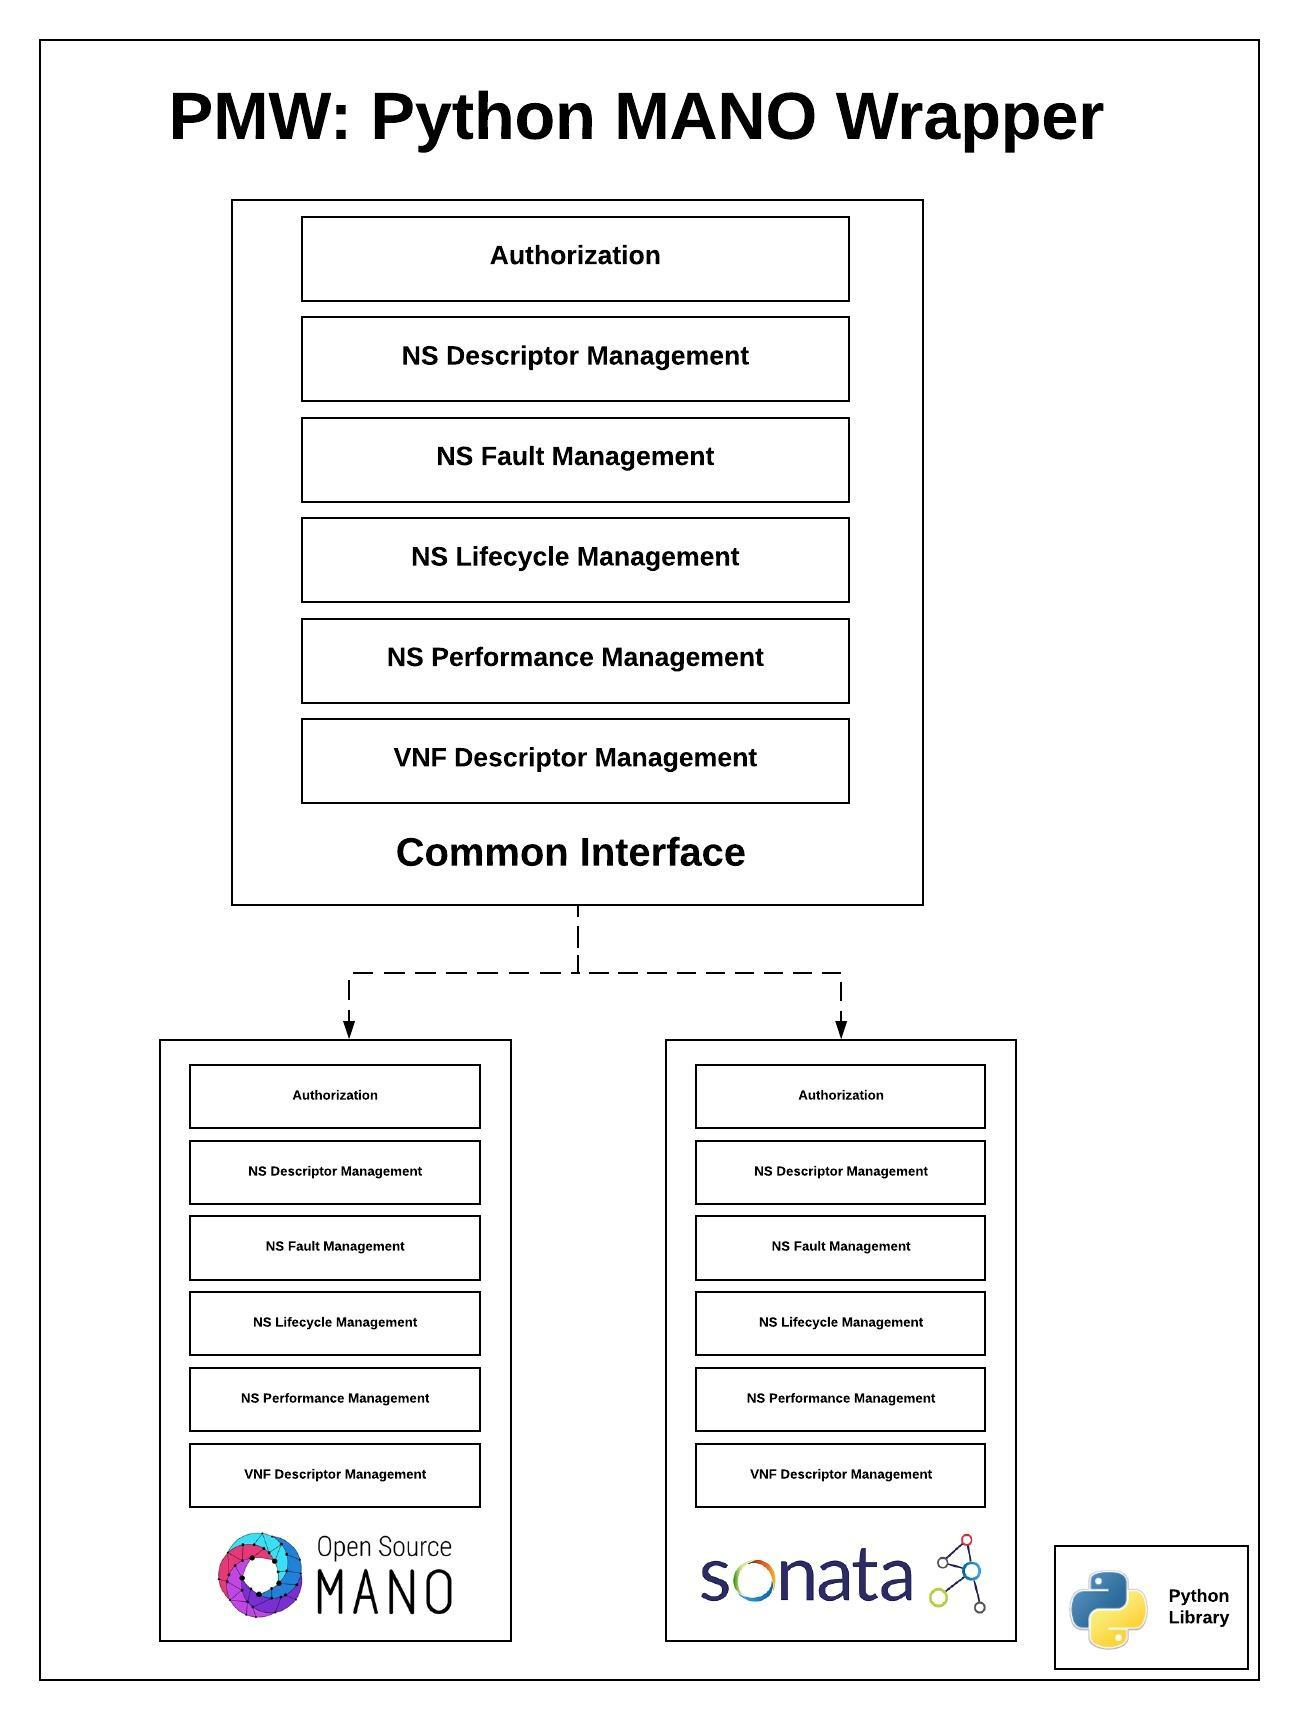
\includegraphics[width=1\linewidth]{figures/WrapperArch}
	\caption{}
	\label{fig:wrapperarch}
\end{figure}
